\documentclass[a4paper]{article}

\usepackage{INTERSPEECH2018}
\usepackage{booktabs}
\usepackage{adjustbox}
\usepackage{multirow}

\title{Multilingual Multi-Task Learning for Low-Resource Acoustic Modeling}

\name{Josh Meyer$^1$}
%The maximum number of authors in the author list is twenty. If the number of contributing authors is more than twenty, they should be listed in a footnote or in acknowledgement section, as appropriate.
\address{
  $^1$University of Arizona}
\email{joshua.richard.meyer@gmail.com}

\begin{document}

\maketitle
% 
\begin{abstract}
  
\end{abstract}
\noindent\textbf{Index Terms}: speech recognition, multi-task learning, acoustic modeling

\section{Introduction}

Previous work has shown that performance for a low-resource language on speech recognition can be improved by adding training data from another, resource-rich language. Typically, data from another language is added as a separate task in the Multi-Task Learning framework via an additional output layer (Caruana 1997).

The targets for this addititional language have always been states of context-dependent triphones, defined by some tree clustering algorithm. This current research builds off the intuition that triphones encode information which is too fine-grained to be maximally useful for language-transfer. Using a higher-level of linguistic abstraction (eg. the monophone), we are able to better extract the kind of language-general information useful in training an acoustic model for some target language.

To put it another way, if we want to lower Word Error Rates for a language like Urdu, learning to distinguish different versions of English [th] in context is probably not very useful. A better way to make use of English data would be to focus on distinguishing more common linguistic contrasts like [p vs b]. In adding an additional language as an auxialilary task, it would be better to focus on distinctions which are robust and will transfer well to a new, target language.


The tasks are created by redefining the parameters of the HMM-GMM system used to bootstrap a DNN-hybrid system, such that the phonetic decision tree is cut short.

The target language is Kyrgyz, and the source language is English. Both data come from audiobooks, English being from LibriSpeech and Kyrgyz from the Bizdin.kg project.




\section{Background Literature}

Past attempts at MTL


\section{DNN-Hybrid Training as Model Transfer}

The standard DNN-Hybrid approach requires the GMM-HMM system to provide the labels for supervised training. This reliance of the DNN on GMM alignments is actually a form of model transfer, where the DNN is trained to perform the extact same classification as its GMM predecessor. The DNN not only learns the frame alignments from the individual GMMs, but also the DNN indirectly learns the structure of the phonetic decision tree used to define the tied-state system. This is because the output layer of the DNN is trained to predict targets which were defined via leaves of the decision tree.


\begin{figure}[!htb]
  \centering
\minipage{0.5\textwidth}
  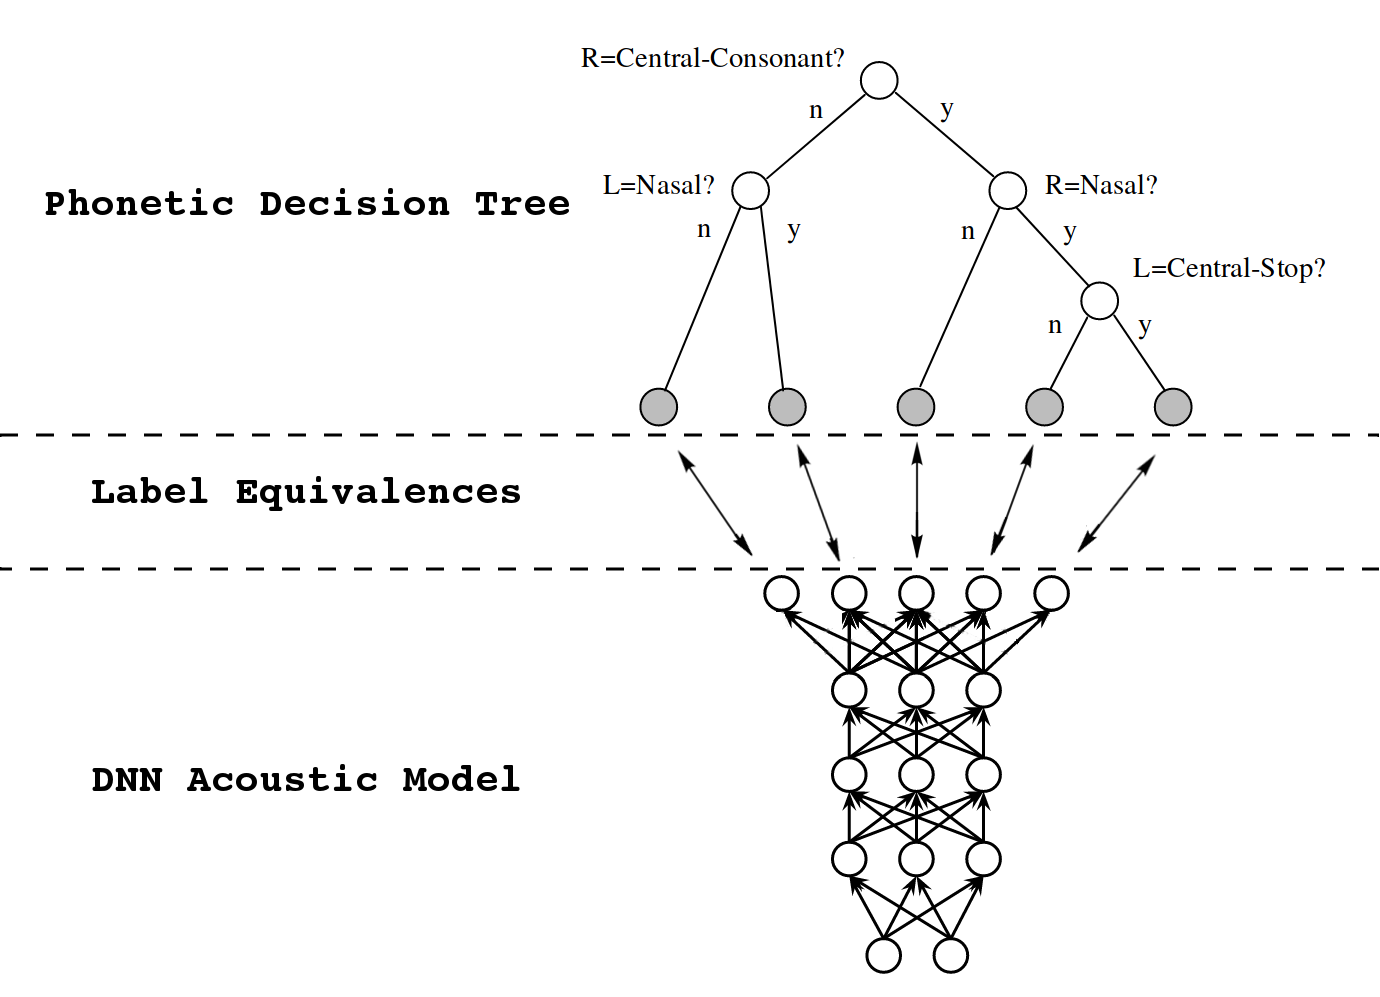
\includegraphics[width=\linewidth]{figs/tree-net.png}
  \caption{GMM$\rightarrow$DNN Model Transfer}
\endminipage\hfill
\end{figure}


Given that standard triphones encode very fine-grained information which may not help performance on a target language, the following experiments investigate GMM$\rightarrow$DNN model transfer at a higher level for an additional source language. 


\section{Experiments}

\subsection{Data}

Two speech corpora are used in the following experiments:

\begin{enumerate}
\item LibriSpeech selection (5 hours)
\item Kyrgyz audiobook section (1.5 hours)
\end{enumerate}

\subsection{Model Building}

All models were build using the Kaldi \texttt{nnet3} approach. The scripts used in this paper can be found at (XXX). These scripts are based on the offical repo multilingual Babel scripts here (XXX).

In GMM training, monophones were allotted a total of 1000 Gaussian components and trained over 25 iterations of EM. These monophones were then expanded into context-dependent triphones via a phonetic decision tree, with a maximum of 1000 leaves (ie. tied-states). The resulting leaves (state clusters) are then trained as context-dedendent triphones with a total of 2000 Gaussian components over 25 iterations of EM.

Given the alignments from the GMM-HMM models, a 5-layer, 200-dimensional TDNN is trained over 5 epochs of backprop on a single GPU instance.

Each auxiliary task is implemented as a separate output layer along with a penultimate hidden layer. All other hidden layers are trained in parallel. 

\subsubsection{English}

Using the standard CMUDict phoneset, 3-state monophones are trained from a flat-start via EM training, and then expanded into triphones via Kaldi's decision tree.

\subsubsection{Kyrgyz}

The Kyrgyz phoneset can be found here (XXX). The transcriptions are basically a simple grapheme set, with predictable variation (allophony) explicitly encoded. For example, the letter K is pronounced as [q] in the context of back vowels, and in the context of front vowels it is pronounced [k]. The phoneme set includes both [q] and [k].

Decoding is performed with a bigram backoff language model was trained on a Wikipedia Kyrgyz dump, and contains, 103,998 unigrams and 56,6871 bigrams.



Because I am interested in the application of this MTL technique to low resource languages, I examine how much the performance boost from the source language changes with regards to the size of the training data for the target language.


\textbf{Baseline}

All the following architectures will be compared to the performance of the following baseline.

To account for any advantage mutliple output layers may bring about, the baseline also contains two output layers, where the tasks are identical. In this way, random initializations in the weights and biases for each task are accounted for.

During testing, \textit{only one} of the tasks (ie. the main task) is used. The additional tasks are dropped and the baseline Kyrgyz triphones are used in decoding. This highlights the purpose of the extra tasks: to force the learning of robust representations in the hidden layers during training. The tasks may in fact not be the best option for final classification; they serve as ``training wheels'' which are then removed once the net is ready.


\textbf{Auxiliary Tasks}

The auxiliary tasks all related to the English language data from the LibriSpeech corpus. Investigating the intuition that labels generated by a standard triphone phonetic decision tree are not the best representation of data for transfer learning, the auxiliary tasks here investigate different levels in the decision tree's branches. By forcing the neural net to recognize higher levels in the tree, we will learn representations which are more abstract, and therefore more likely to be relevant multi-lingually. 

\subsection{Results}


All results are performed on the same held-out section of Kyrgyz audiobook. The bigram language model, lexicon, and main-task decision tree are build into a standard decoding graph in the traditional Kaldi style.

5-layer, 500 dimensial hidden layer, 10 epoch results:


\begin{figure}[!htb]
  \centering
\minipage{0.5\textwidth}
  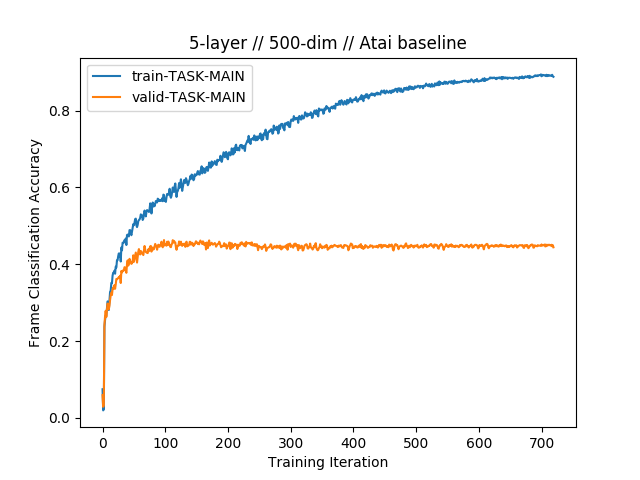
\includegraphics[width=\linewidth]{figs/atai-baseline.png}
  \caption{Baseline Model}
\endminipage\hfill
\end{figure}

As we can see, the baseline model overfits to the training data after about 250 iterations. The performance for the final model (clearly would be beat out if we used early stopping) is 53.66\% WER on decoding the held-out test data.



\begin{figure}[!htb]
  \centering
\minipage{0.5\textwidth}
  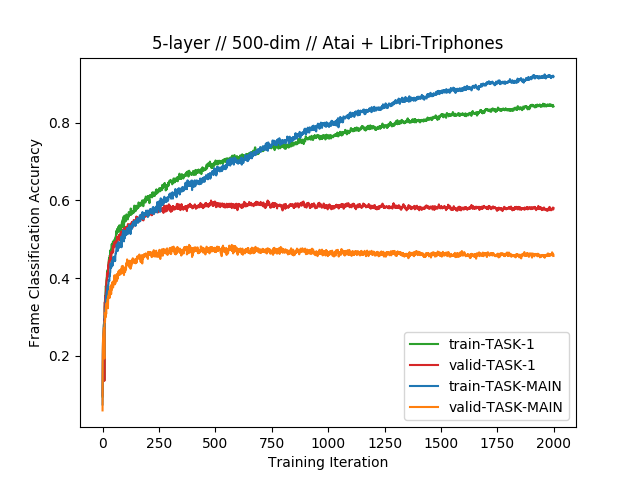
\includegraphics[width=\linewidth]{figs/atai-libritriphones.png}
  \caption{Aux Task == LibriSpeech Triphones}
\endminipage\hfill
\end{figure}


\begin{figure}[!htb]
  \centering
\minipage{0.5\textwidth}
  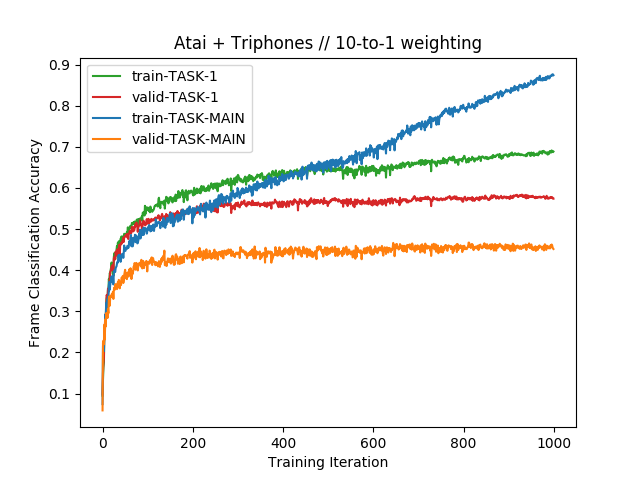
\includegraphics[width=\linewidth]{figs/atai-libritriphones-10-to-1.png}
  \caption{Aux Task == LibriSpeech + Triphones // 10-to-1}
\endminipage\hfill
\end{figure}



Above, we see the addition of triphones as an auxiliary task from the LibriSpeech corpus. Overfit to Atai after 500 iterations. The performance for the final model (clearly would be beat out if we used early stopping) is 49.85\% WER on decoding the held-out test data.

\begin{figure}[!htb]
  \centering
\minipage{0.5\textwidth}
  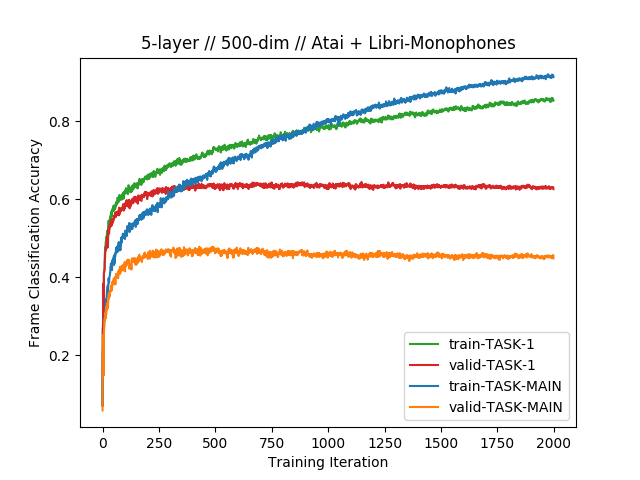
\includegraphics[width=\linewidth]{figs/atai-librimonophones.png}
  \caption{Aux Task == LibriSpeech Monophones}
\endminipage\hfill
\end{figure}


Finally, monophones from the LibriSpeech corpus. Overfit to Atai after 500 iterations. The performance for the final model (clearly would be beat out if we used early stopping) is 51.32\% WER on decoding the held-out test data.



Here we are with the last model:


\begin{figure}[!htb]
  \centering
\minipage{0.5\textwidth}
  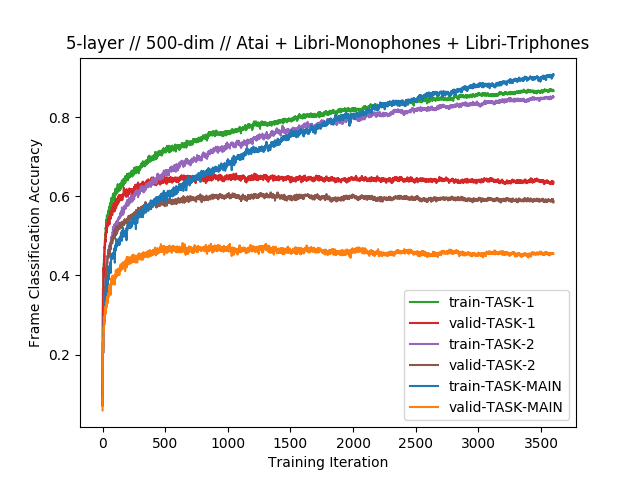
\includegraphics[width=\linewidth]{figs/atai-libritriphones-librimonophones.png}
  \caption{Aux Task == LibriSpeech Monophones + Triphones}
\endminipage\hfill
\end{figure}






\begin{table}[!htbp]
  \centering
  \begin{adjustbox}{width=.45\textwidth}
    \begin{tabular}{lc}
      \toprule
      \textbf{Tasks} & \textbf{WER\%}\\
      \midrule
      Atai (STL Baseline) &  53.66\% \\
      Atai + Libri-Triphones & 49.85\%  \\
      Atai + Libri-Triphones 10-to-1 & 50.54\%  \\
      Atai + Libri-Monophones &  51.32\% \\
      Atai + Libri-Monophones + Libri-Triphones & 51.32\%  \\
      \bottomrule
    \end{tabular}
    \label{table:data}
  \end{adjustbox}
  
  \caption{Experimental Setup}
  
\end{table}



Takeaways from 500-dim // 5-epoch // 2-to-1 weighting:

\begin{enumerate}
\item Addition of LibriSpeech beats out Kyrgyz-only.
\item Triphones work better than monophones
\item Both languages / tasks overfit
\item best triphone model beats best baseline (ie. early stopping)
\item atai overfit slower with additional tasks
\item atai overfits with monophones earlier, I think because it's an easier task
\item 10-to-1 weighting on 5 epochs seems like we've overfit the data, but validation is STILL increaing... try to run on 10 epochs and see what happens. 500 dim, 5 layer, aux task == triphones.
\item try 5-to-1, because 2-to-1 seems too weak, and 10-to-1 seems too strong
\end{enumerate}




\section{Discussion}


\section{Conclusions}

\section{Acknowledgements}


\bibliographystyle{IEEEtran}

\bibliography{mybib}

% \begin{thebibliography}{9}
% \bibitem[1]{Davis80-COP}
%   S.\ B.\ Davis and P.\ Mermelstein,
%   ``Comparison of parametric representation for monosyllabic word recognition in continuously spoken sentences,''
%   \textit{IEEE Transactions on Acoustics, Speech and Signal Processing}, vol.~28, no.~4, pp.~357--366, 1980.
% \bibitem[2]{Rabiner89-ATO}
%   L.\ R.\ Rabiner,
%   ``A tutorial on hidden Markov models and selected applications in speech recognition,''
%   \textit{Proceedings of the IEEE}, vol.~77, no.~2, pp.~257-286, 1989.
% \bibitem[3]{Hastie09-TEO}
%   T.\ Hastie, R.\ Tibshirani, and J.\ Friedman,
%   \textit{The Elements of Statistical Learning -- Data Mining, Inference, and Prediction}.
%   New York: Springer, 2009.
% \bibitem[4]{YourName17-XXX}
%   F.\ Lastname1, F.\ Lastname2, and F.\ Lastname3,
%   ``Title of your INTERSPEECH 2018 publication,''
%   in \textit{Interspeech 2018 -- 19\textsuperscript{th} Annual Conference of the International Speech Communication Association, September 2-6, Hyderabad, India Proceedings, Proceedings}, 2018, pp.~100--104.
% \end{thebibliography}

\end{document}
